
\section{Overview} % Bookmark information, displayed in the progress tree

\subsection{SIGMOD At a Glance}
\begin{frame}[red] %hmm.. thought i could change colour here :S
\frametitle{Submissions}

\begin{itemize} 
 \item Keynotes
      \begin{itemize} 
      \item Analytic Database Technologies for a New Kind of User - The Data Enthusiast, by Pat Hanrahan (Stanford)
      \item Symbiosis in Scale Out Networking and Data Management, by Amin Vahdat (UCSD and Google)
      \end{itemize}
 \item 16 Research sessions (+10 PODS sessions)

 \item 6 Industry sessions
\end{itemize}

\end{frame}


\begin{frame}[red] %hmm.. thought i could change colour here :S
\frametitle{Awards}

      \begin{itemize} 
      \item SIGMOD Test-of-Time Awards
      \begin{itemize}
	\gitem Executing SQL over Encrypted Data in the Database-Service-Provider Model
	\ritem Visionary paper on "Database as a service" focusing on how to use cloud services while keeping some information hidden from the cloud service provider
      \end{itemize}
      \end{itemize}

      \begin{itemize} 
      \item SIGMOD Best Paper Award
      \begin{itemize}
	\gitem High-Performance Complex Event Processing over XML Streams
	\ritem Introduced XSeq, an XPath extension orders of magnitude more efficient than existing XML engines.
      \end{itemize}
      \end{itemize}

\end{frame}



\subsection{Topics}
\begin{frame}[red] %hmm.. thought i could change colour here :S
\frametitle{Topics} 

      \begin{itemize} 
      \ritem Social Networks and Graph Databases
      \begin{itemize} 
      \item Partitioning, Clustering, subgraph isomorphism
      \end{itemize}
      \ritem Temporal and Graph Databases
      \begin{itemize} 
      \item 2 on querying graphs, 1 on temporal alignment of queries
      \end{itemize} % no prints
      \ritem Mobile Databases
      \begin{itemize} 
      \item 2 papers on Privacy, 1 on caching
      \end{itemize}
      \gitem Distributed and Parallel Databases
      \gitem Social Media and Crowdsourcing
      \gitem Modern RDBMSs
      \end{itemize}
\end{frame}





% 
% 
% 
% 
% 
% \subsection{Problem}
% \begin{frame}[red] %hmm.. thought i could change colour here :S
% \frametitle{How do we express the Cache Performance?}
% 
%   Benefit is expected cost saved:
%     \begin{itemize}
%     \item On server: computation time
%     \item On proxy: communication time
%     \end{itemize}
% 
% \vspace{1.5em}
% 
% We need to answer:
% \begin{itemize}
%     \itemsep -2pt
%     \item Which queries $Q_{s,t}$ can be answered by the path $P_{a,b}$?
%     \item For query $Q_{s,t}$, what are the cost savings?
% \end{itemize}
% 
% \vspace{1.5em}
%   Given a: 
%     \begin{itemize}
%     \item Cache Size Budget 
%     \item Query Log
%     \end{itemize}
%   Then build a cache $\Psi$ with max benefit $\gamma(\Psi)$\\
% \end{frame}
% 
% 
% \begin{frame}[color=red] %hmm.. thought i could change colour here :S
%     \begin{figure}
%     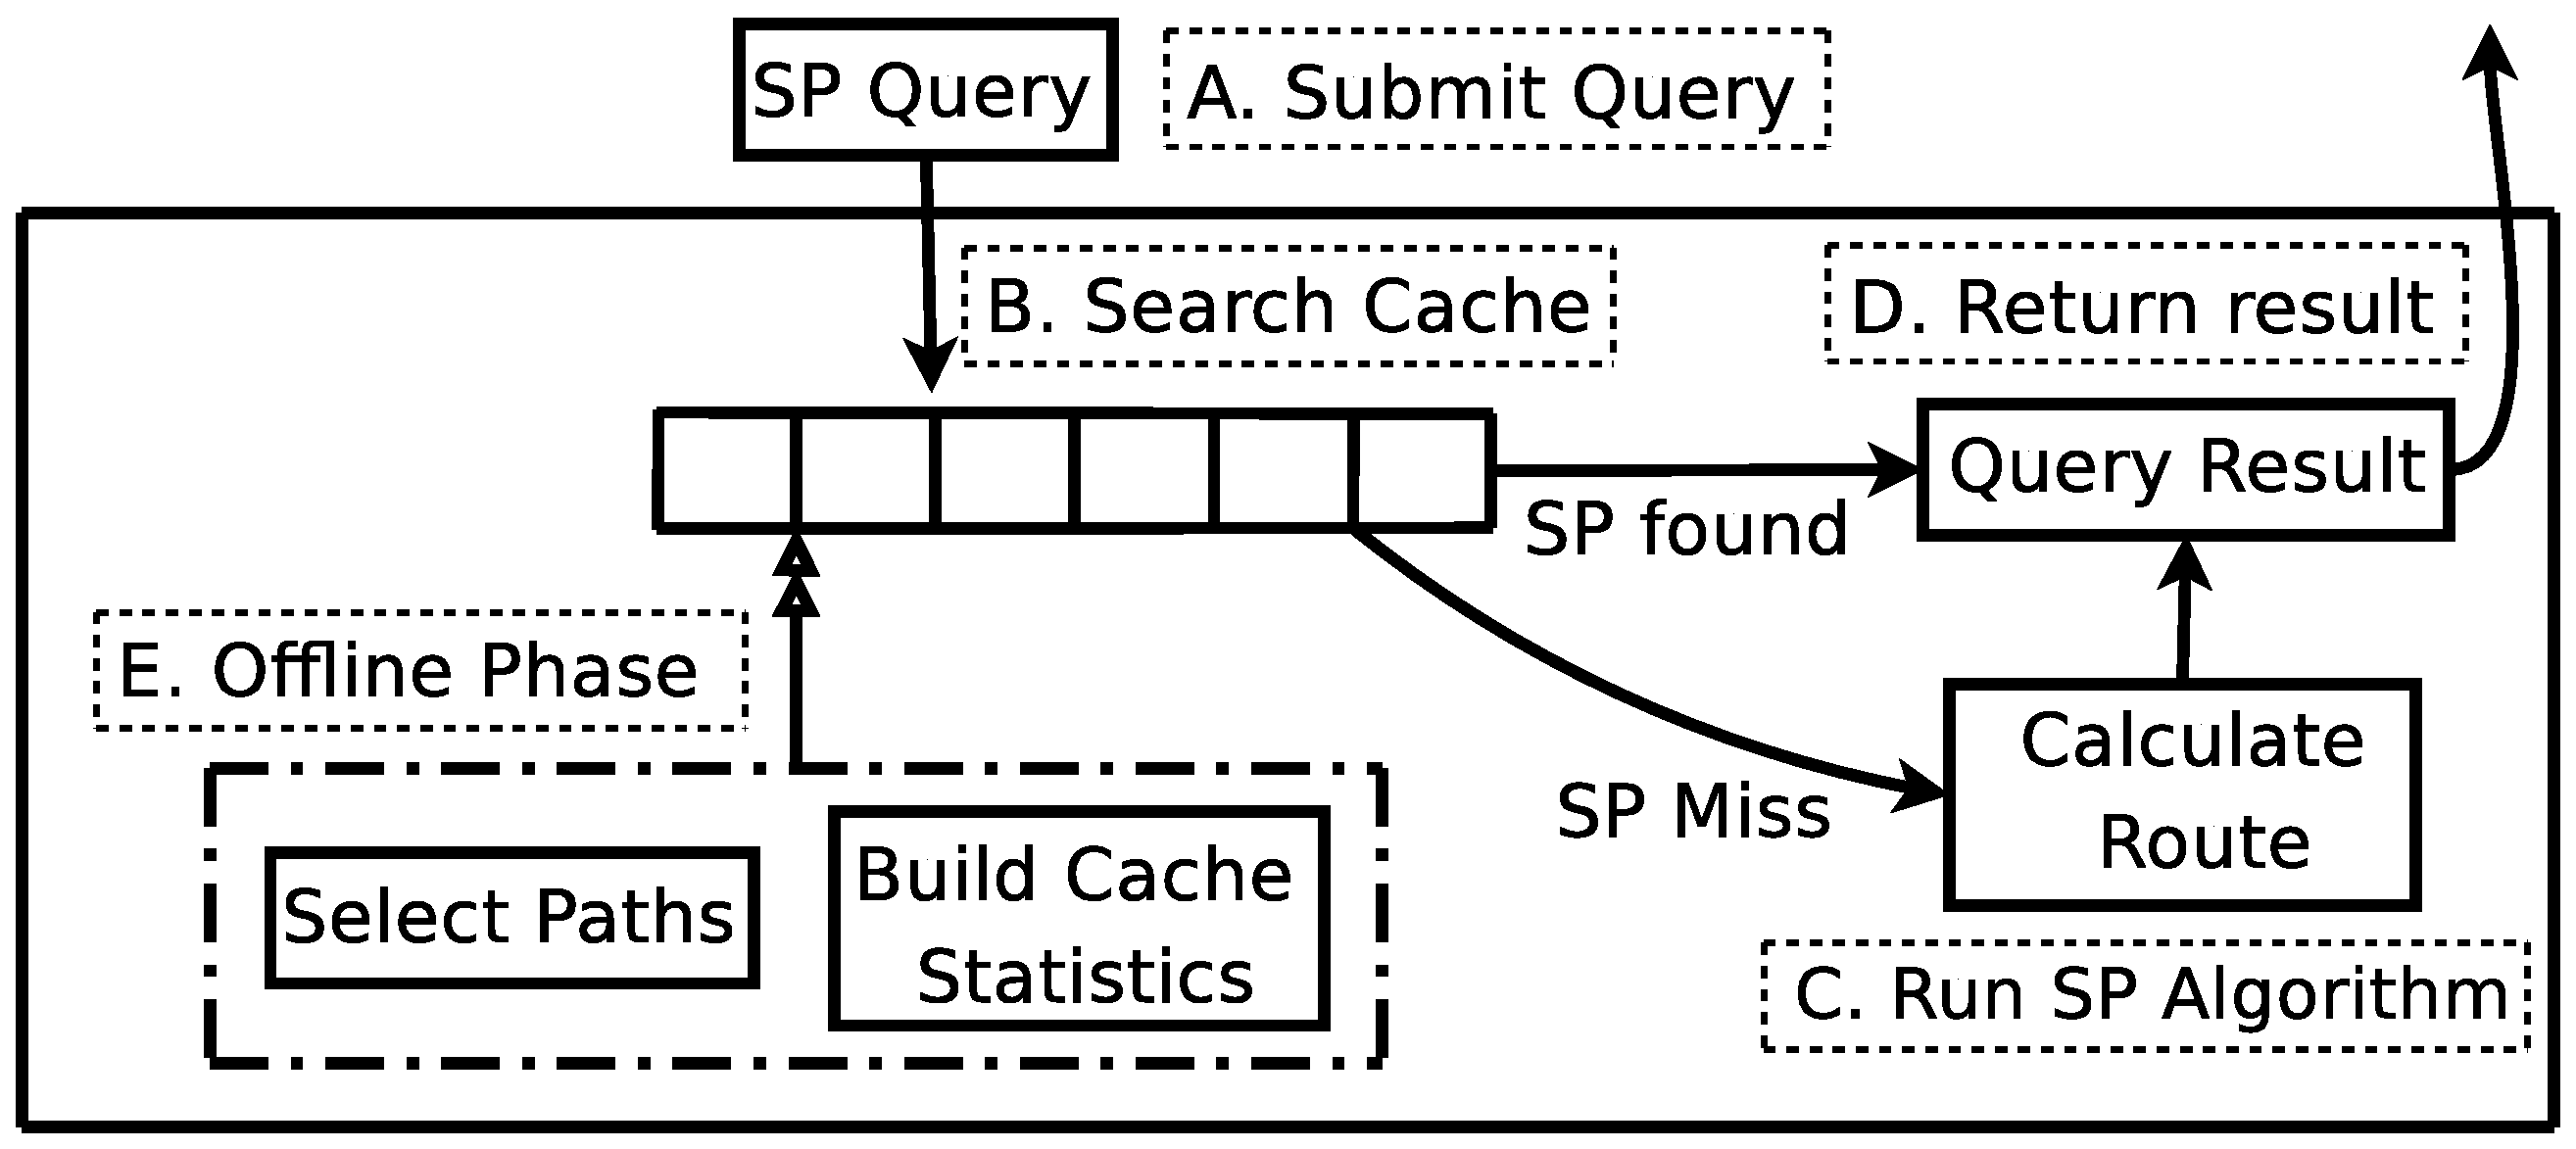
\includegraphics[width=1.05\textwidth]{images/routequery} 
%     \
%     \end{figure}
% 
% \begin{columns}
%   \begin{column}{0.5\textwidth}
%     \vspace{-0.8em}
%     \begin{itemize}
%     \itemsep -2pt
%       \item Systematic model for benefit
%       \item Techniques for query log statistics extraction 
%     \end{itemize}
%   \end{column}
%   \begin{column}{0.6\textwidth}
%     \vspace{-1.3em}
%     \begin{itemize}
%      \itemsep -2pt
%       \item Efficient caching structure
%       \item Shortest Path benchmarking techniques
%     \end{itemize}
%   \end{column}
% \end{columns}
% \end{frame}
% 
% 
% 
% 
